% Methods section (merged from methodology, empirical models, and algorithm)

\subsection{Experimental Design}

We conduct experiments on both synthetic and real-world networks to understand the relationship between sampling parameters and accuracy. We generate three synthetic network topologies representing archetypal urban forms---trellis (dense grid), tree (dendritic/suburban), and linear (corridor)---each as a $3 \times 3$ tile pattern with approximately 2940m extent (Figure~\ref{fig:topologies}). For validation, we extract street networks from OpenStreetMap for London (Soho), Madrid (Centro), and Phoenix (Scottsdale).

\begin{figure}[htbp]
    \centering
    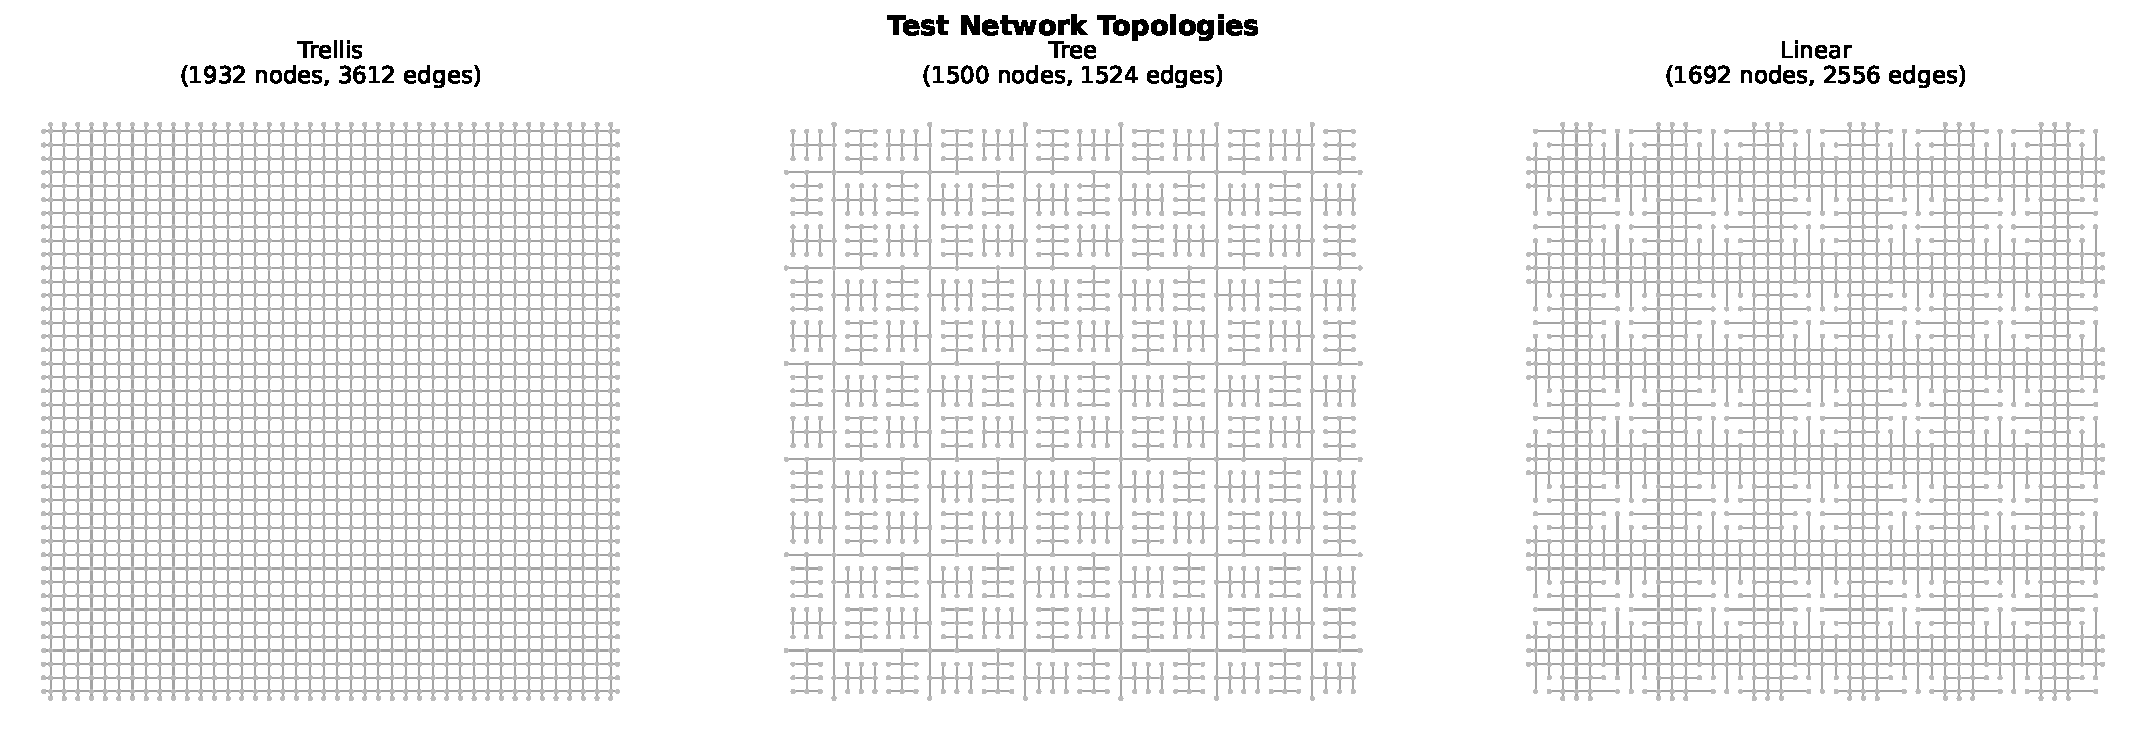
\includegraphics[width=\textwidth]{figures/topologies.pdf}
    \caption{Synthetic network topologies: trellis, tree, and linear.}
    \label{fig:topologies}
\end{figure}

We compute two localised centrality measures: harmonic closeness (sum of inverse distances to nodes within threshold) and betweenness (count of shortest paths through each node). Both metrics support shortest-path and angular distance heuristics; we focus on shortest-path computation, with angular results in the supplementary material. When estimating centrality from a sample of source nodes, we use the H\'{a}jek estimator \citep{Hajek1971}, which scales by the ratio of population size $N$ to actual sample size $n$.

Our primary accuracy metric is Spearman's rank correlation coefficient ($\rhosp$) between true and estimated centrality values. Ranking accuracy is most relevant for urban analysis, where researchers identify high- or low-centrality locations rather than interpreting absolute values. The key insight motivating our approach is that accuracy depends on \emph{effective sample size}:
\begin{equation}
    \effn = \bar{R} \times p
    \label{eq:effective_n}
\end{equation}
where $\bar{R}$ is the mean reachability (average number of nodes reachable within the distance threshold) and $p$ is the sampling probability.

\subsection{Empirical Accuracy Models}

We fit empirical models predicting accuracy from effective sample size. After comparing four functional forms (see Appendix~A for model comparison), we select the hyperbolic form for its desirable asymptotic properties ($\rhosp \to 1$ as $\effn \to \infty$):
\begin{equation}
    \rhosp = 1 - \frac{A}{B + \effn}
    \label{eq:rho_model}
\end{equation}
We fit separate models for harmonic closeness and betweenness, and for shortest-path and angular distances, as these exhibit different accuracy characteristics. We fit the 10th percentile conditional quantile using quantile regression \citep{Koenker1978} to ensure 90\% of network configurations meet or exceed predicted accuracy.

\input{tables/model_parameters}

The relationship between harmonic closeness and betweenness sample requirements varies by distance heuristic: for shortest paths, harmonic closeness requires approximately \ratioHBShortest$\times$ more samples than betweenness; for angular paths, betweenness requires approximately \ratioBHAngular$\times$ more samples than harmonic closeness.

\begin{figure}[htbp]
    \centering
    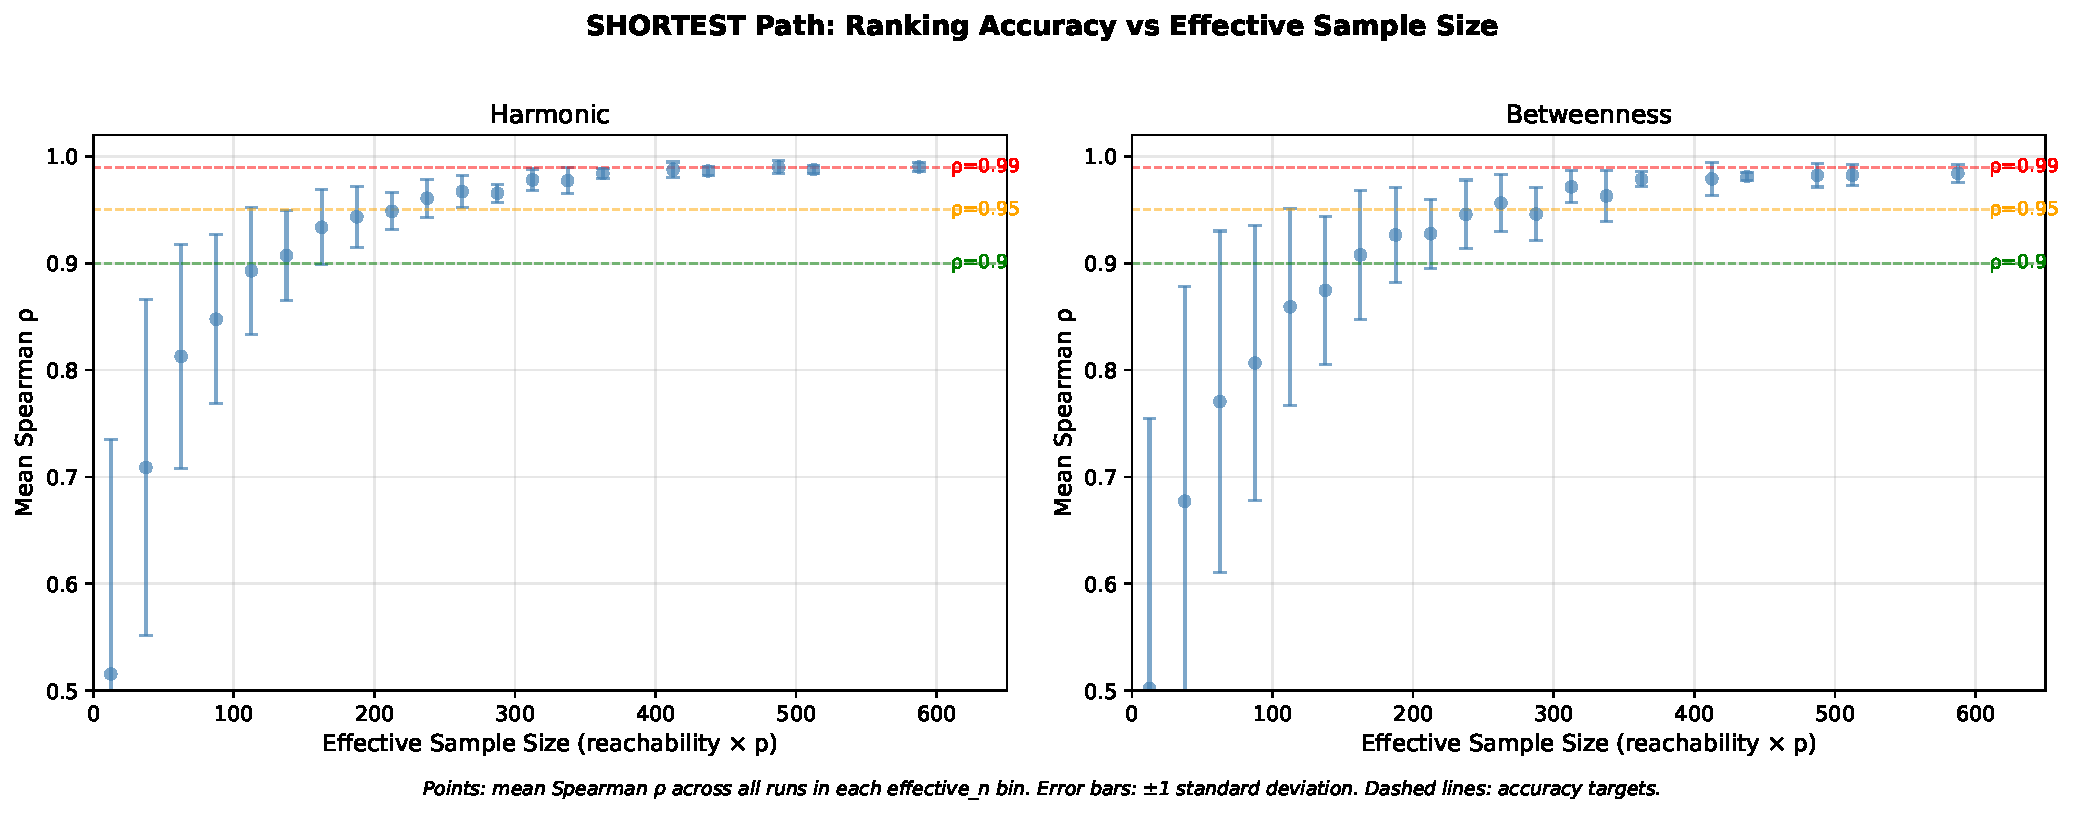
\includegraphics[width=\textwidth]{figures/accuracy_vs_effn_shortest.pdf}
    \caption{Observed Spearman $\rhosp$ versus effective sample size for shortest path distances. Left: harmonic closeness. Right: betweenness. Points coloured by network topology. Solid lines show fitted models (10th percentile).}
    \label{fig:accuracy_vs_effn_shortest}
\end{figure}

Inverting Equation~\ref{eq:rho_model}, the required sampling probability for target accuracy $\rhosp^*$ is:
\begin{equation}
    p^* = \frac{1}{\bar{R}} \left( \frac{A}{1 - \rhosp^*} - B \right)
    \label{eq:required_p}
\end{equation}
We also fit models for uncertainty (standard deviation) following the expected $1/\sqrt{n}$ convergence. The relationship between relative and absolute CI-width is discussed in Appendix~A.

\begin{figure}[htbp]
    \centering
    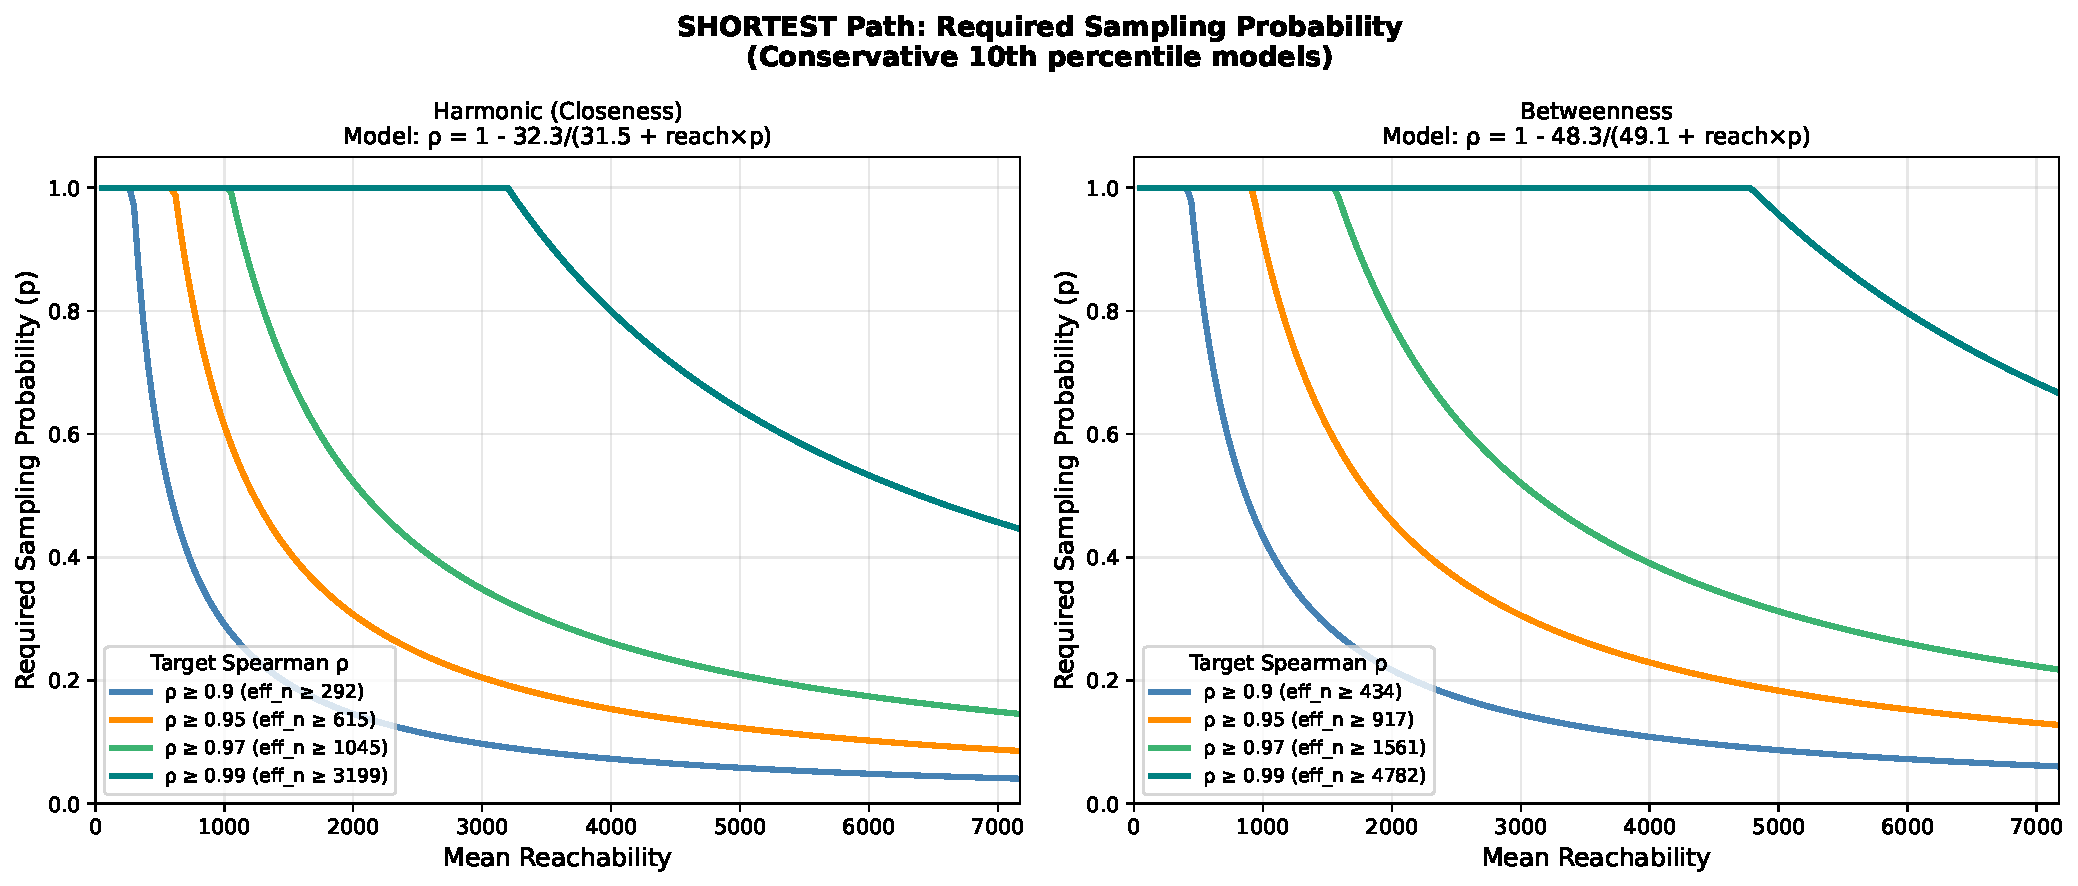
\includegraphics[width=\textwidth]{figures/required_probability_shortest.pdf}
    \caption{Required sampling probability for shortest path distances to achieve target accuracy levels as a function of mean network reachability. Based on the betweenness (conservative) model.}
    \label{fig:required_probability_shortest}
\end{figure}

\subsection{Adaptive Sampling Algorithm}

Given a network $G = (V, E)$, distance thresholds $\{r_1, \ldots, r_d\}$, and target accuracy $\rhosp^*$, the goal is to compute localised centrality at each threshold with guaranteed accuracy while minimising computation time. Uniform sampling fails because short distances have low reachability (insufficient $\effn$) while long distances waste computation on unnecessary precision. The adaptive approach resolves this tension by calibrating sampling probability independently for each distance threshold.

The algorithm operates in three phases. In the first phase, reachability probing, we estimate mean reachability by running Dijkstra's algorithm from a small sample of nodes (default: 50) and counting reachable nodes at each distance threshold. In the second phase, probability computation, we use Equation~\ref{eq:required_p} to compute the required sampling probability for each distance. Short distances yield $p_i \to 1.0$; long distances enable $p_i \ll 1.0$. In the third phase, per-distance execution, we process each threshold $r_i$ by sampling source nodes with probability $p_i$, running centrality computation, and scaling results by $1/p_i$.

As distance increases, so too does the speedup (Figure~\ref{fig:speedup}).

\begin{figure}[htbp]
    \centering
    \includegraphics[width=\textwidth]{figures/speedup_vs_distance.pdf}
    \caption{Computation time (left) and speedup factor (right) for adaptive sampling compared to full computation. Speedup increases with distance as higher reachability enables more aggressive sampling. Madrid network; averaged over 5 runs.}
    \label{fig:speedup}
\end{figure}
